\begin{figure*}[ht!]\centering
	\newcounter{groupcount}
	\pgfplotsset{
		legend style={at={(axis cs:21,0)},anchor=south west},
		draw group line/.style n args={5}{
			after end axis/.append code={
				\setcounter{groupcount}{0}
				\pgfplotstableforeachcolumnelement{#1}\of\datatable\as\cell{%
					\def\temp{#2}
					\ifx\temp\cell
					\ifnum\thegroupcount=0
					\stepcounter{groupcount}
					\pgfplotstablegetelem{\pgfplotstablerow}{X}\of\datatable
					\coordinate [yshift=#4] (startgroup) at (axis cs:\pgfplotsretval,0);
					\else
					\pgfplotstablegetelem{\pgfplotstablerow}{X}\of\datatable
					\coordinate [yshift=#4] (endgroup) at (axis cs:\pgfplotsretval,0);
					\fi
					\else
					\ifnum\thegroupcount=1
					\setcounter{groupcount}{0}
					\draw [
					shorten >=-#5,
					shorten <=-#5
					] (startgroup) -- node [anchor=base, yshift=0.5ex] {#3} (endgroup);
					\fi
					\fi
				}
				\ifnum\thegroupcount=1
				\setcounter{groupcount}{0}
				\draw [
				shorten >=-#5,
				shorten <=-#5
				] (startgroup) -- node [anchor=base, yshift=0.5ex] {#3} (endgroup);
				\fi
			}
		}
	}
	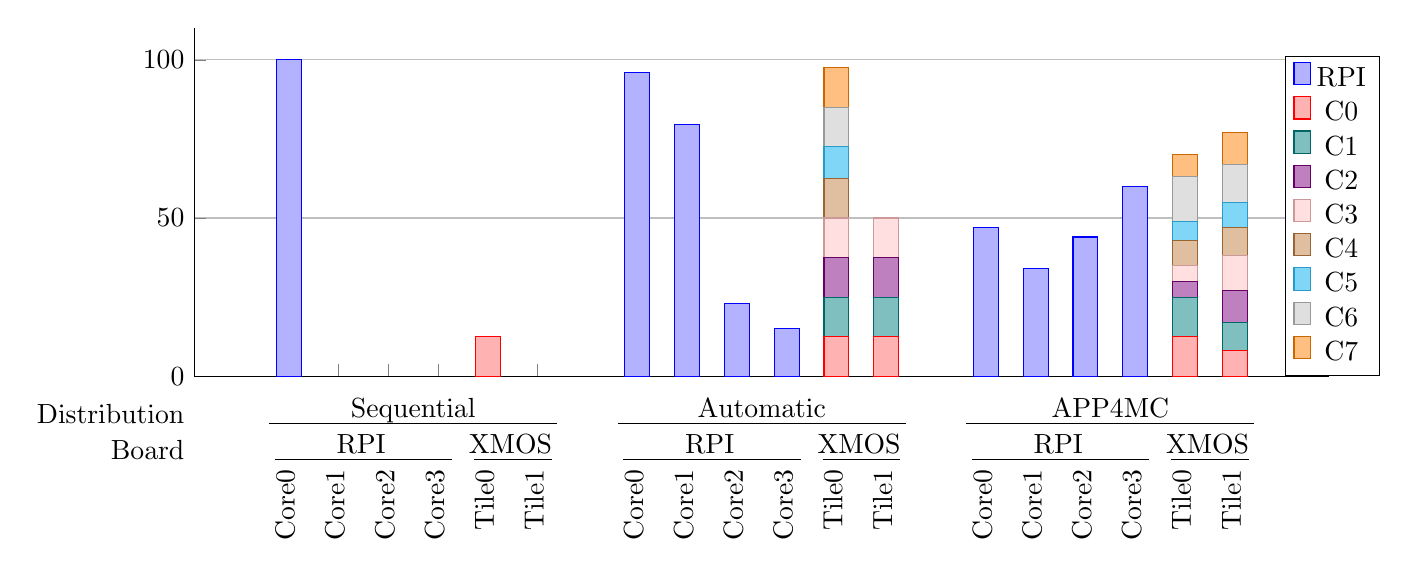
\begin{tikzpicture}%NO COMMENTS ALLOWED IN PGFPLOT VALUES
	\pgfplotstableread{
		X Gp D1 Name RPI C0 C1 C2 C3 C4 C5 C6 C7
		1 Sequential RPI Core0 100 0 0 0 0 0 0 0 0 
		2   Sequential RPI Core1 0 0 0 0 0 0 0 0 0
		3   Sequential RPI Core2 0 0 0 0 0 0 0 0 0
		4   Sequential RPI Core3 0 0 0 0 0 0 0 0 0
		5   Sequential XMOS Tile0 0 12.5 0 0 0 0 0 0 0 
		6   Sequential XMOS Tile1 0 0 0 0 0 0 0 0 0 
		8 Automatic RPI Core0 96 0 0 0 0 0 0 0 0
		9  Automatic RPI Core1 79.6 0 0 0 0 0 0 0 0
		10  Automatic RPI Core2 22.9 0 0 0 0 0 0 0 0
		11  Automatic RPI Core3 15.1 0 0 0 0 0 0 0 0
		12  Automatic XMOS Tile0 0 12.5 12.5 12.5 12.5 12.5 10 12.5 12.5 
		13  Automatic XMOS Tile1 0 12.5 12.5 12.5 12.5 0 0 0 0
		15  APP4MC RPI Core0 47 0 0 0 0 0 0 0 0
		16  APP4MC RPI Core1 34 0 0 0 0 0 0 0 0
		17  APP4MC RPI Core2 44 0 0 0 0 0 0 0 0
		18  APP4MC RPI Core3 60 0 0 0 0 0 0 0 0
		19  APP4MC XMOS Tile0 0 12.5 12.5 5 5 8 6 14 7 
		20  APP4MC XMOS Tile1 0 8 9 10 11 9 8 12 10 
	}\datatable
	\begin{axis}[
	axis lines*=left, ymajorgrids,
	width=16cm, height=6cm,
	ymin=0,
	ybar stacked,
	bar width=9pt,
	xtick=data,
	xticklabels from table={\datatable}{Name},
	xticklabel style={rotate=90,xshift=-7ex,anchor=mid east},
	draw group line={D1}{RPI}{RPI\,}{-7ex}{5pt},
	draw group line={D1}{XMOS}{XMOS\,}{-7ex}{5pt},
	draw group line={Gp}{Sequential}{Sequential}{-4ex}{7pt},
	draw group line={Gp}{Automatic}{Automatic}{-4ex}{7pt},
	draw group line={Gp}{APP4MC}{APP4MC}{-4ex}{7pt},
	after end axis/.append code={
		\path [anchor=base east, yshift=0.ex]
		(rel axis cs:0,0) node [yshift=-7ex] {Board}
		(rel axis cs:0,0) node [yshift=-4ex] {Distribution};
	}
	]
	
	\addplot table [x=X, y=RPI] {\datatable}; \addlegendentry{RPI}
	\addplot table [x=X, y=C0] {\datatable}; \addlegendentry{C0}
	\addplot [teal!80!black,fill=teal!50!white] table [x=X, y=C1]{\datatable}; \addlegendentry{C1}
	\addplot [violet!80!black,fill=violet!50!white] table [x=X, y=C2]{\datatable}; \addlegendentry{C2}
	\addplot [pink!80!black,fill=pink!50!white] table [x=X, y=C3]{\datatable}; \addlegendentry{C3}
	\addplot [brown!80!black,fill=brown!50!white] table [x=X, y=C4]{\datatable}; \addlegendentry{C4}
	\addplot [cyan!80!black,fill=cyan!50!white] table [x=X, y=C5]{\datatable}; \addlegendentry{C5}
	\addplot [lightgray!80!black,fill=lightgray!50!white] table [x=X, y=C6]{\datatable}; \addlegendentry{C6}
	\addplot [orange!80!black,fill=orange!50!white] table [x=X, y=C7]{\datatable}; \addlegendentry{C7}
	\end{axis}
	\end{tikzpicture}
	\vspace{-20pt}
	\caption{Core utilization in \% (y-axis) for sequentail, automatic, and APP4MC distribution}
	\label{fig:dischart}
\end{figure*}